
\subsection{Resumen de objetivos}


\normalfont

El trabajo práctico consiste en el análisis de la compensación de la misma fuente de alimentación lineal realimentada que en el anterior trabajo práctico (\textbf{TP1A}). El análisis es por simulación con \textbf{SPICE} (\textbf{LTSPICE} específicamente en nuestro caso), de donde se pretende validar los valores de las redes de compensación.


\subsection{Desarrollo}

Se hace un análisis cualitativo de la compensación de la fuente, para luego pasar a la validación de las redes de compensación. La validación se realiza variando el valor de los componentes a un valor por debajo y uno por encima del valor elegido en el diseño, y comparando como varía el comportamiento de la fuente de tres maneras distintas. En primer lugar se observa como varía la ganancia de lazo con la frecuencia, esta simulación se realiza utilizando el circuito mostrado en la figura~ \figref{fig:fig_complete_circuit_loop}, haciendo un barrido en frecuencia y simulando en forma paramétrica con los valores a comparar, observando los márgenes de fase y de ganancia, lo cuál nos da una idea de la estabilidad lograda en cada caso. En segundo lugar se observa la respuesta en frecuencia a lazo cerrado, esta simulación se realiza utilizando el circuito mostrado en la figura~ \figref{fig:fig_complete_circuit_rf}, igual que antes se realiza un barrido en frecuencia y simulando en forma paramétrica con los valores a comparar, observando el ancho de banda obtenido y otras características de la respuesta, como ser picos que indiquen posibles inestabilidades y como varía la fase. Por último se analiza la respuesta temporal de la fuente de alimentación al cargar y descargar bruscamente la misma, esta simulación se realiza utilizando el circuito mostrado en la figura~ \figref{fig:fig_complete_circuit_step}, esta simulación nos permite observar posibles oscilaciones y sobre-picos que se produzcan a la salida de la fuente, viendo el efecto que tiene la variación de los valores de las redes de compensación, la simulación se repite para cada valor que se ensaya. Cada una de las simulaciones mencionadas anteriormente se realiza en los dos modos posibles de funcionamiento de la fuente, con el lazo de tensión activo y con el lazo de corriente activo, a su vez se simulan dos casos distintos para cada modo, alterando los valores de los resistores de configuración y el valor de la carga, viendo como varía la salida en cada caso.


\clearpage


\begin{figure}[H] %htb
\begin{center}
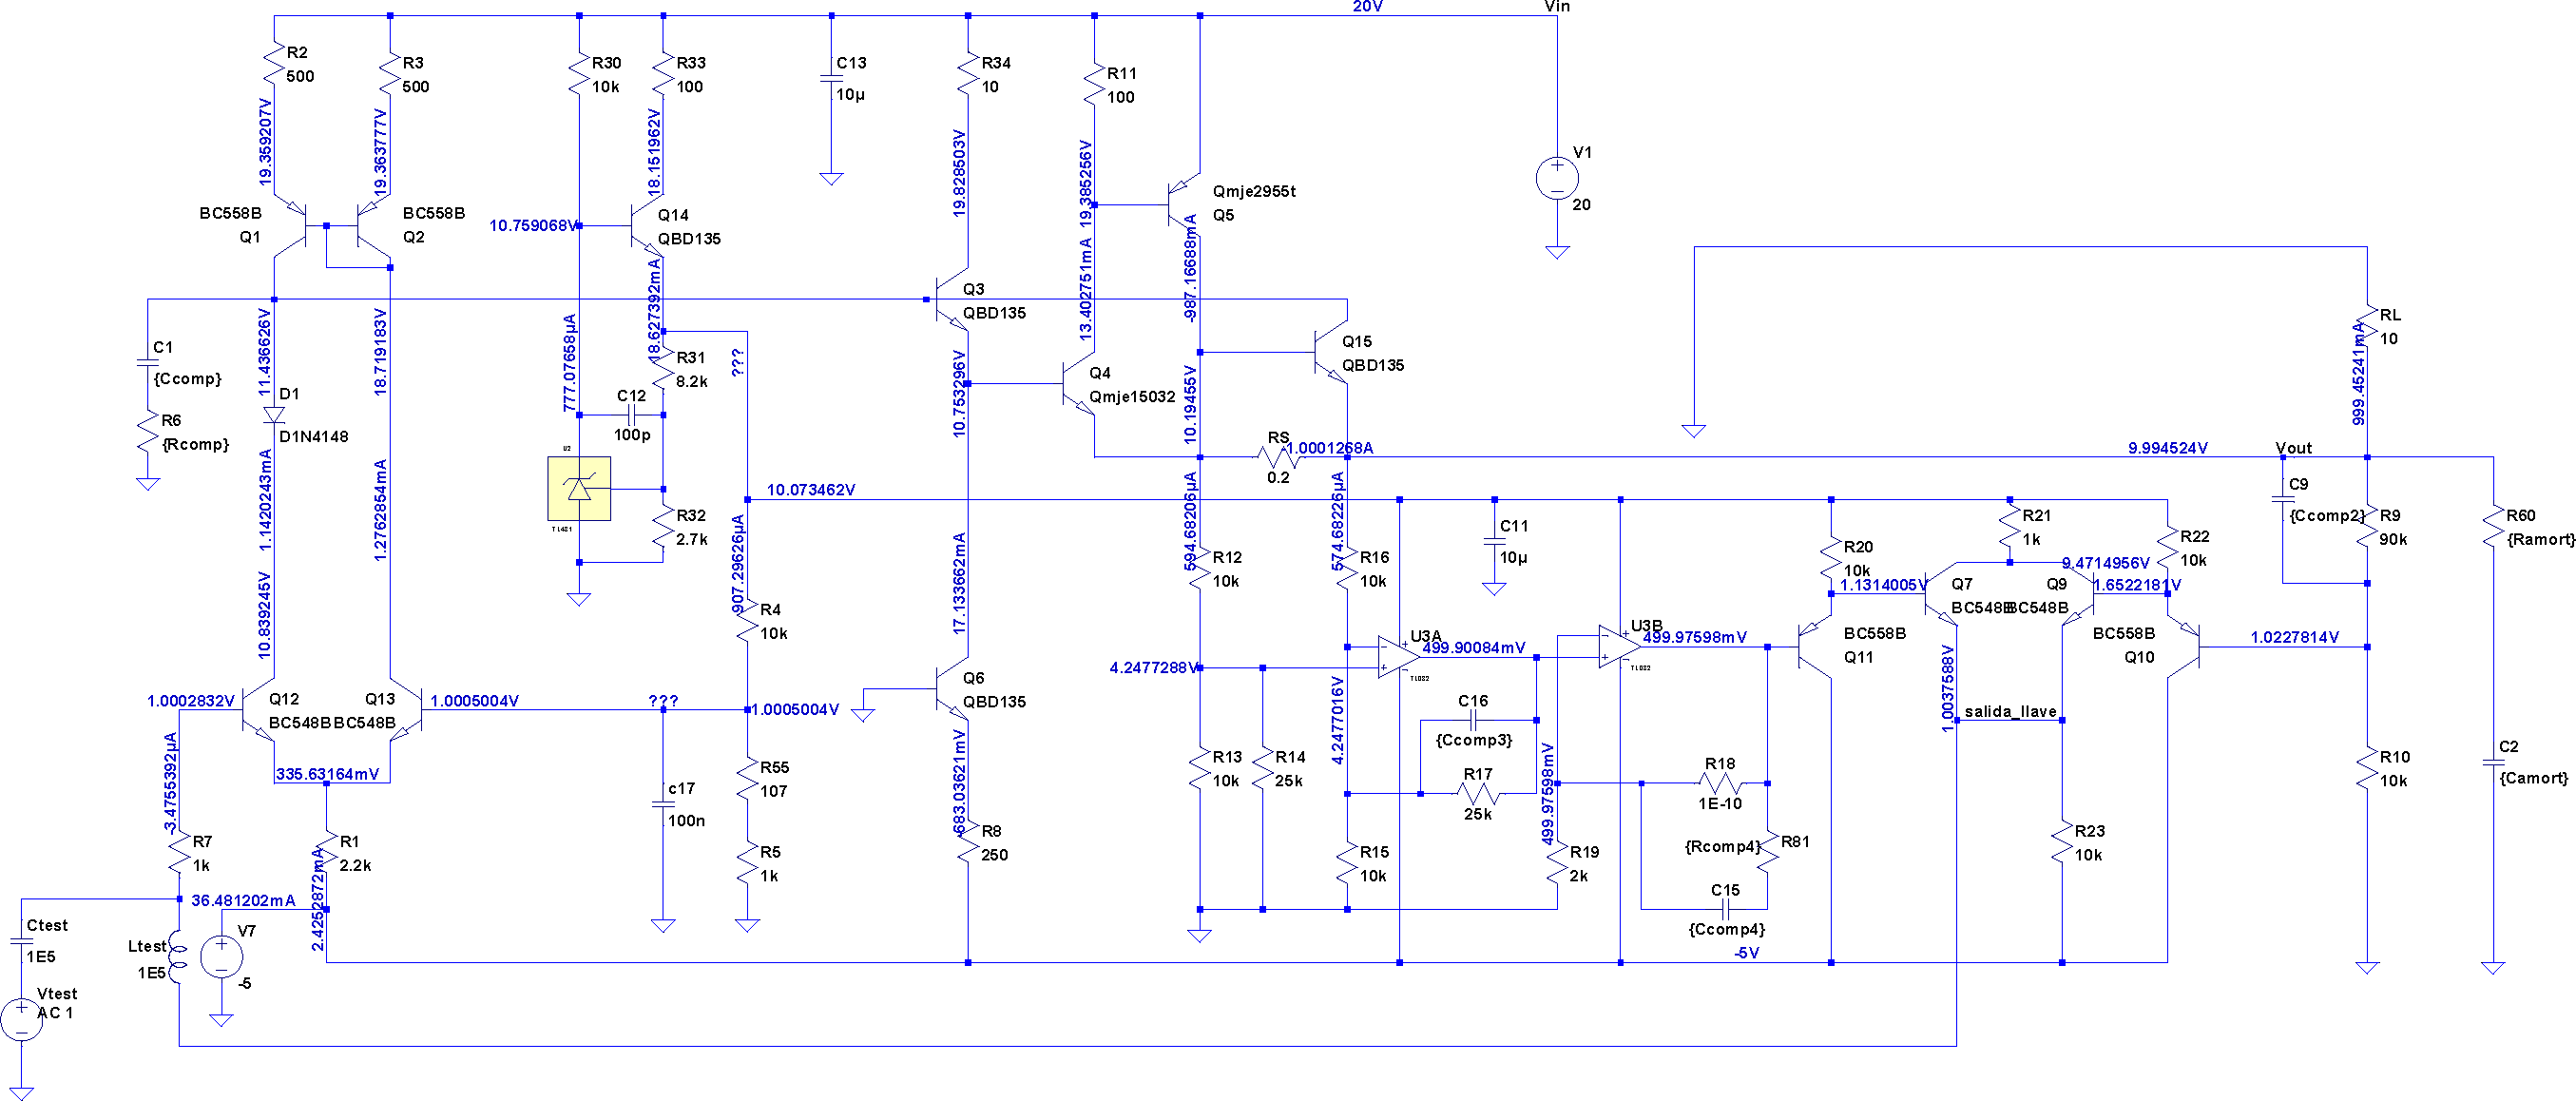
\includegraphics[width=1.2 \textwidth, angle=90]{./img/desarrollo/power_supply_LOOP.png}
\caption{\label{fig:fig_complete_circuit_loop}\footnotesize{Circuito utilizado para la obtención de la ganancia de lazo en función de la frecuencia.}}
\end{center}
\end{figure}

\clearpage

\begin{figure}[H] %htb
\begin{center}
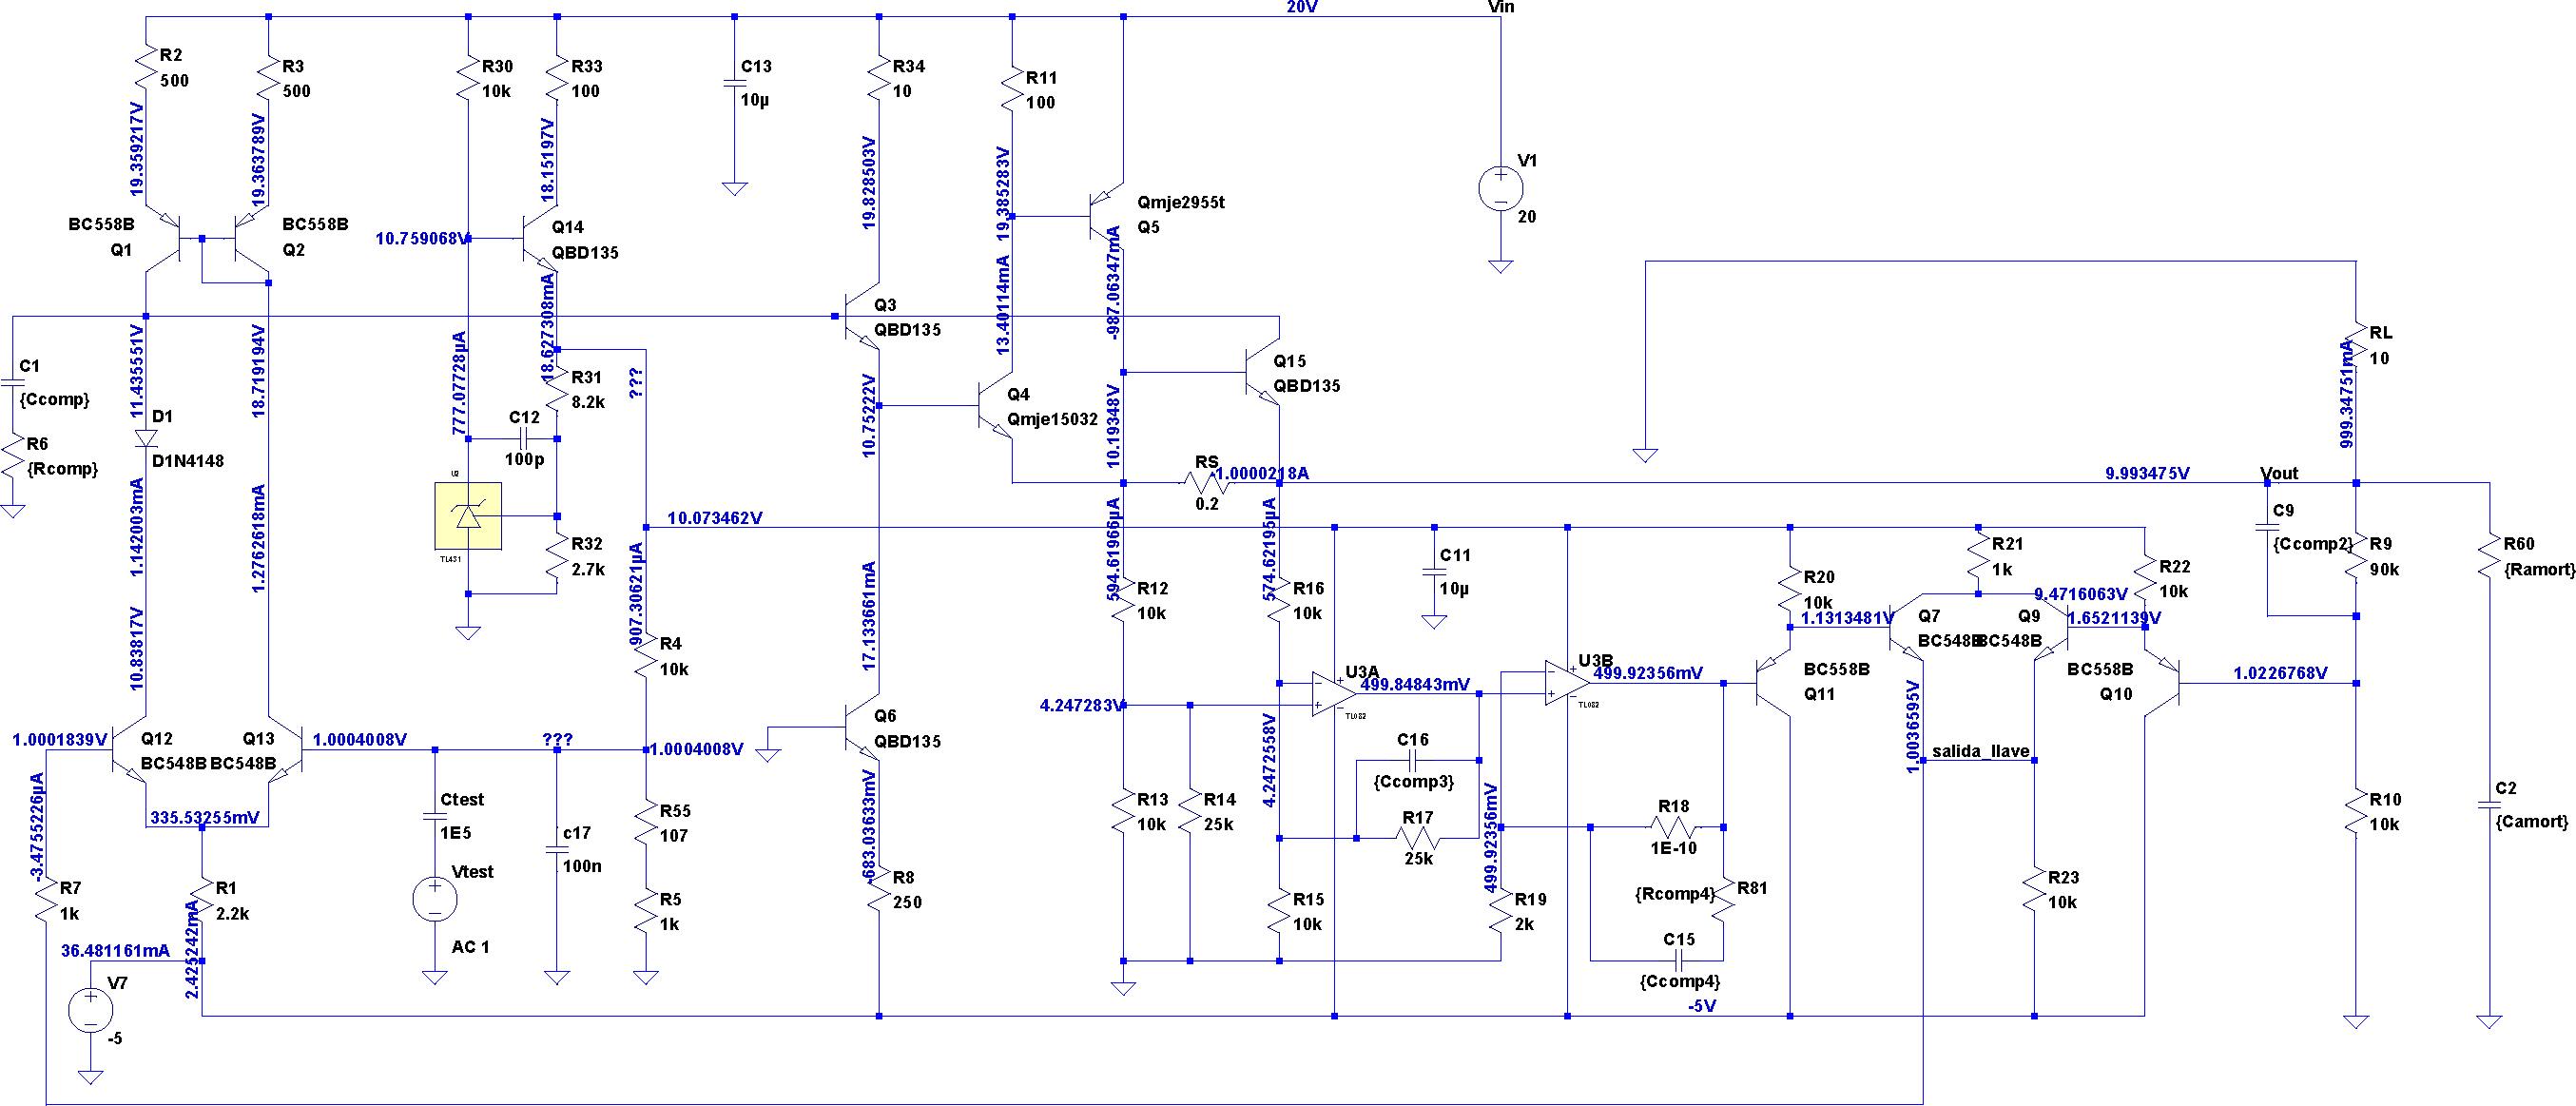
\includegraphics[width=1.2 \textwidth, angle=90]{./img/desarrollo/power_supply_RF.png}
\caption{\label{fig:fig_complete_circuit_rf}\footnotesize{Circuito utilizado para la obtención de la respuesta en frecuencia.}}
\end{center}
\end{figure}

\clearpage

\begin{figure}[H] %htb
\begin{center}
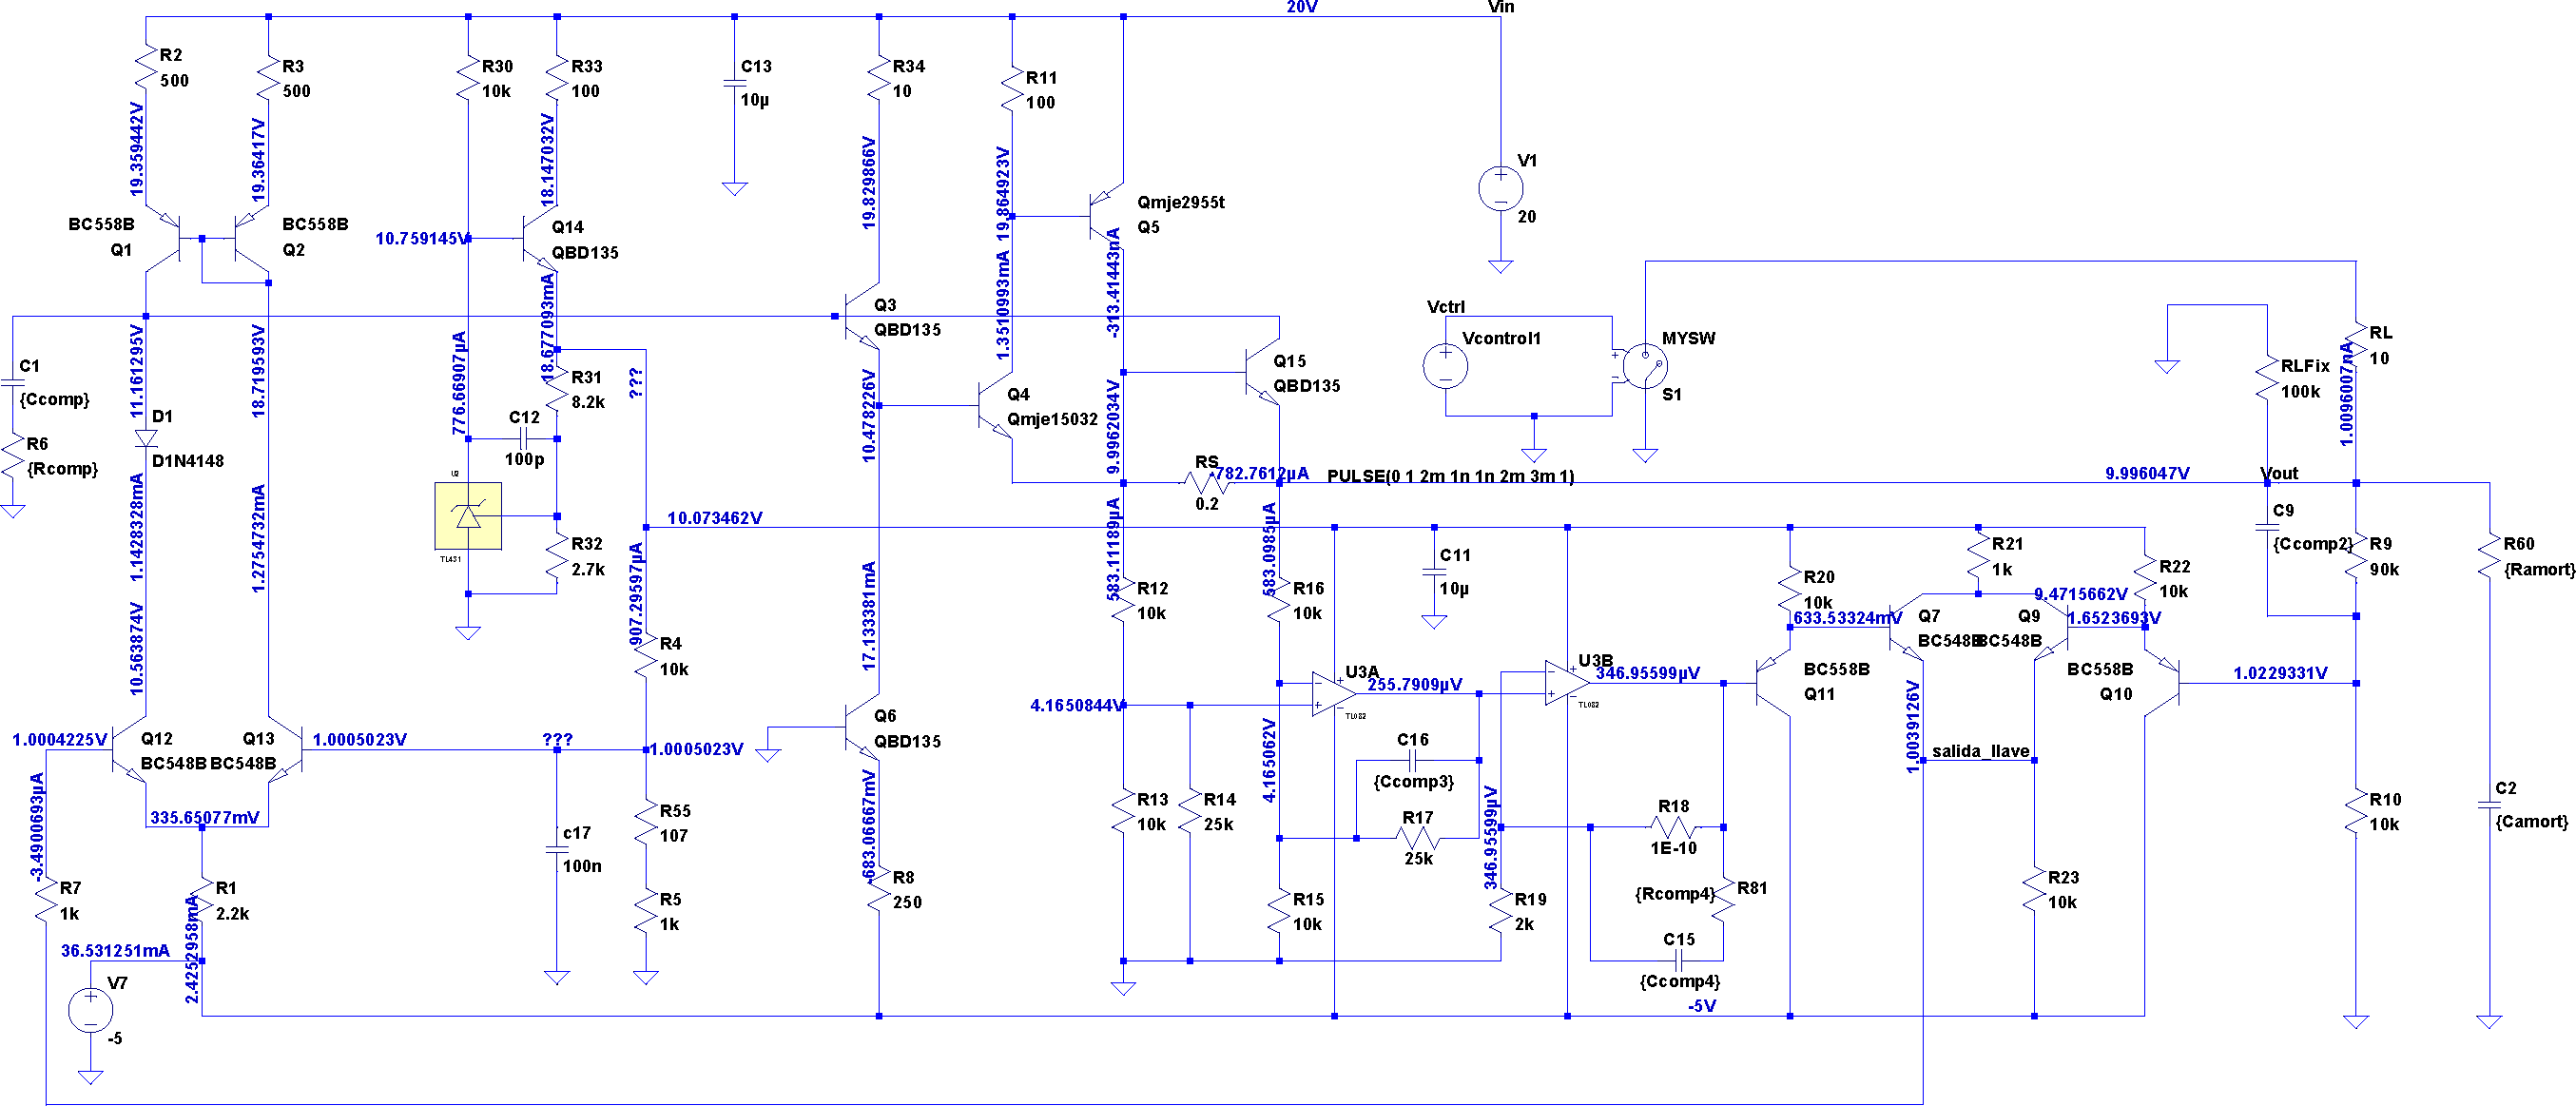
\includegraphics[width=1.2 \textwidth, angle=90]{./img/desarrollo/power_supply_STEP.png}
\caption{\label{fig:fig_complete_circuit_step}\footnotesize{Circuito utilizado para la obtención de la respuesta dinámica.}}
\end{center}
\end{figure}